% !TEX TS-program = pdflatex
% !TEX encoding = UTF-8 Unicode

% This is a simple template for a LaTeX document using the "article" class.
% See "book", "report", "letter" for other types of document.

\documentclass[11pt]{article} % use larger type; default would be 10pt

\usepackage[utf8]{inputenc} % set input encoding (not needed with XeLaTeX)

%%% Examples of Article customizations
% These packages are optional, depending whether you want the features they provide.
% See the LaTeX Companion or other references for full information.

%%% PAGE DIMENSIONS
\usepackage{geometry} % to change the page dimensions
\geometry{a4paper} % or letterpaper (US) or a5paper or....
\geometry{margin=2cm} % for example, change the margins to 2 inches all round
% \geometry{landscape} % set up the page for landscape
%   read geometry.pdf for detailed page layout information


\usepackage{setspace}
\setstretch{1.5}

\usepackage{graphicx} % support the \includegraphics command and options
\graphicspath{ {./img/} }

\usepackage{biblatex} %Imports biblatex package
\addbibresource{sources.bib} %Import the bibliography file

% \usepackage[parfill]{parskip} % Activate to begin paragraphs with an empty line rather than an indent

%%% PACKAGES
\usepackage{booktabs} % for much better looking tables
\usepackage{array} % for better arrays (eg matrices) in maths
\usepackage{paralist} % very flexible & customisable lists (eg. enumerate/itemize, etc.)
\usepackage{verbatim} % adds environment for commenting out blocks of text & for better verbatim
\usepackage{subfig} % make it possible to include more than one captioned figure/table in a single float
% These packages are all incorporated in the memoir class to one degree or another...

\usepackage{amsmath}
\usepackage{float}

%%% HEADERS & FOOTERS
\usepackage{fancyhdr} % This should be set AFTER setting up the page geometry
\pagestyle{fancy} % options: empty , plain , fancy
\renewcommand{\headrulewidth}{0pt} % customise the layout...
\lhead{}\chead{}\rhead{}
\lfoot{}\cfoot{\thepage}\rfoot{}

%%% SECTION TITLE APPEARANCE
\usepackage{sectsty}
\allsectionsfont{\sffamily\mdseries\upshape} % (See the fntguide.pdf for font help)
% (This matches ConTeXt defaults)

%%% ToC (table of contents) APPEARANCE
\usepackage[nottoc,notlof,notlot]{tocbibind} % Put the bibliography in the ToC
\usepackage[titles,subfigure]{tocloft} % Alter the style of the Table of Contents
\renewcommand{\cftsecfont}{\rmfamily\mdseries\upshape}
\renewcommand{\cftsecpagefont}{\rmfamily\mdseries\upshape} % No bold!

%%% END Article customizations

%%% The "real" document content comes below...

\title{Final project report\\
	   Portfolio optimization}
\author{Juha Reinikainen}
%\date{} % Activate to display a given date or no date (if empty),
         % otherwise the current date is printed 

\begin{document}
\maketitle

\section{Problem}

Portfolio optimization involves deciding how to use the available investment budget to maximize the total value of the investment and minimize its risk \cite{van2021parden}. Maximizing social responsibility can also be included as one of the goals \cite{chen2021social}. The investment budget is allocated to assets which can be for example stocks, gold, foreign exchange, real estate, bonds and cryptocurrencies \cite{faizan2019multiobjective}. For simplicity only stocks are considered in this project.

The problem is difficult because there is a large number of possible assets to include in the portfolio and even larger number of ways to divide the budget among them. Investing also has a lot of uncertainty as stock prices are affected by real world events which are hard to capture in the model \cite{du2020new}.


\section{Modelling}

The problem can be modelled as a three objective optimization problem maximing expected return of the investment, minimizing its risk and maximizing social responsibility.

Data-driven approach to this problem involves predicting expected return and risk based on historical time-series data of stock prices over given time range, possibly years. Stock price can be sampled e.g. daily, weekly, monthly or quaterly. The stocks that are included in the data-set need to be selected.


\subsection{Variables}

The decision vector consist of proportions of total budget allocated to n stocks $w = (w_1, w_2, ..., w_n)$ and binary variable for each stock which indicates whether the corresponding stock is included in the portfolio $y=(y_1, y_2,..., y_n)$. 

\subsection{Constraints}

It's assumed that the whole budget is used so the sum of weights should add up to one for the weight where the corresponding boolean flag is 1.

Boundary constraint requires that the weights of each stock is between $w_{min}$ and $w_{max}$. Maximum limit makes it so that all budget is not allocated to too small number of stocks leading to diverse portfolio. Too small weights typically have little impact on the performance and weak liquidity and can be costly in respect to brokerage fess or monitoring costs \cite{ertenlice2018survey}.

Cardinality constraint requires that the number of stocks included in the portfolio is between some two numbers $C_{min}$ and $C_{max}$. 

\subsection{Objectives}

Popular way to model these objectives is Markowitz model which is also known as mean-variance model \cite{kolm201460}. The risk measure from that model is used. For predicting the prices of individual stocks ARIMA model is used. ARIMA is a popular time series prediction model which also has been used in portfolio optimization \cite{kumar2021multi}. 

Given time series data of n stocks for time period of 0...T with stock price p(t, i) of stock i at time t. prices of stock i are a series $x_i$.

$x_i = (p(0, i), p(1, i), ..., p(T, i))$\\

Prices can be computed into future for wanted number of steps using ARIMA with time series data as input. ARIMA depends of three parameters: p,d,q. p is the order of the auto-regressive model (AR), d is the degree of differencing (I) and q is the order of moving average (MA) model. Since there are 50 models to be trained (for each stock), these parameters are optimized using lbfgs optimizer to find good parameters from range 0-5 for these three parameters.

This gives us a new series.

$x_i^{future} = (p(T+1, i), p(T+2, i), ..., p(T+steps, i))$

Return of an investment for stock i is calculated by.

$roi(i) = \frac{p(T+steps,i) - p(T,i)}{p(T,i)}$

\textbf{Expected return} for portfolio is calculated as weighted sum of all individual returns.

$er(w,y) = \Sigma_{i=1}^{n} (w_i * y_i * roi(i))$

In markowitz model the risk is modelled using covariance of price change of stocks. n x n square covariance matrix Cov contrains covariances of each roi(i) values. Given weights and inclusion flags, \textbf{The risk} for portfolio is given by.

$risk(w,y) = (w y)^T Cov (w y)$

Third objective included in the problem is social responsibility which can be modelled using environmental, social and governance (ESG) score \cite{chen2021social}. Taking social responsibility into consideration can lead to long-term advantages as risk of a company losing face over its actions is common. There are multiple ways to compute the ESG score and multiple organizations that do it. 

\textbf{The overall social responsibility} value for a portfolio is calculated as weighted sum of stock esg scores and weight of each stock.

$esg(w,y) = \Sigma_{i=1}^n (w_i * y_i * esg_i)$



\subsection{Problem}

Putting all this together the whole problem is.

\begin{equation}
\begin{split}
minimize \{ risk(w,y), -er(w,y), -esg(w,y) \}\\
\Sigma_{i=1}^n (w_i * y_i) = 1\\
w_{min} \leq w_i \leq w_{max}, i = 1...n\\
C_{min} \leq \Sigma_{i=1}^n y_i \leq C_{max}\\
y_i \in \{0,1\}, i = 1...n\
\end{split}
\end{equation}

\section{Data}


The stock price data was collected from Yahoo Finance by calling its api with different stocks and merging these into one dataset. For example the weekly prices between 2021-05-09 20:55:46 and 2022-05-09 20:55:46 can be queried using following url.

\url{https://query1.finance.yahoo.com/v7/finance/download/ADS.DE?period1=1620582946&period2=1652118946&interval=1wk&events=history&includeAdjustedClose=true}

Where perdiod1 and period2 are the start and end times of the range as unix timestamps. The stocks included in the problem where the stocks in eurostoxx 50 index.

For this project the scores were acquired from Kaggle dataset \url{https://www.kaggle.com/datasets/debashish311601/esg-scores-and-ratings?resource=download}. The needed 50 `Overall ESG SCORE'-values for the stocks were then picked from the data. 


\section{Algorithm and settings}

NSGA-II algorithm is used to solve the multiobjective constrained mixed-integer problem. The algorithm is run for 2000 generations with population size 200.

For the first n real variables simulated binary crossover and polynomial mutation are used. For the last n binary variables two-point binary crossover and bitflip mutation are used. Crossover probability is set to 1, mutation probability is set to $\frac{1}{50}$. Distribution index for real mutation and crossover are set to 3. 

The constraint that the weight need to add up to one can be enforced using repair method \cite{kaucic2019portfolio}. The weights are first clamped to $w_{min}$ $w_{max}$ range. Then weight vector is element-wise multiplied by vector y to remove unselected stocks. Then each weight is divided by sum of all weights. It's easy to see that now weights add up to one. Special case where all weights are zero can be handled by assigning all weights with value $\frac{1}{n}$.

\begin{equation}
\begin{split}
&\frac{w_1}{w_1 + w_2 + ... + w_n} + \frac{w_2}{w_1 + w_2 + ... + w_n} + \frac{w_n}{w_1 + w_2 + ... + w_n}\\
&= \frac{w_1 + w_2 + ...  +w_n}{w_1 + w_2 + ... + w_n}\\
&= 1
\end{split}
\end{equation}

$C_{min}$ was set to 6 and $C_{max}$ to 20 to make sure that the budget is allocated to sufficient amount of stocks. $w_{min}$ was set to 0.02 and $w_{max}$ to 0.6. 

The ARIMA models are trained on stock prices data from 1.4.2018 to 1.4.2022. Prediction is done 3 months into future (1.7.2022) with these models to get price prediction. The models are also cross validated using sliding window technique and mean symmetric mean absolute percentage error (SMAPE) score is computed for the models.

\section{Results}

The cross validation scores for each model are given below for each stock as mean of SMAPE values. The errors are mostly below 10\% implying that good enought parameters for ARIMA were found and the model has acceptable accuracy given volatility of the stock market.

After 2000 generations and 400000 function evaluations all the 200 solutions were feasible and nondominated in respect to each other. The algorithm was able to find a diverse set of solutions in respect to all the objectives. Figure 1 shows parallel coordinate plot depicting the 200 solutions in objectives space. Here the tradeoff between objectives is somewhat visibly where high return generally leads to high risk and lower social responsibility even though there are exceptions.

\begin{table}[H]
\begin{tabular}{| c | c | }
\hline
stock    & SMAPE\\
\hline
ADS.DE   & 8.178385746708626\\
ADYEN.AS & 10.641090818052325\\
AD.AS    & 5.408601054821343\\
AI.PA    & 4.786506648996402\\
AIR.PA   & 11.846596331941681\\
ALV.DE   & 7.019777303513461\\
ABI.BR   & 9.809535329106653\\
ASML.AS  & 8.526407784730827\\
CS.PA    & 8.955262184806415\\
BAS.DE   & 7.996981181671698\\
BAYN.DE  & 8.671662640055118\\
BBVA.MC  & 11.018076694228448\\
SAN.MC   & 10.875880871596674\\
BMW.DE   & 8.921097861343082\\
BNP.PA   & 11.041334277715546\\
CRG.IR   & 7.355815124187261\\
BN.PA    & 5.411205090121721\\
DB1.DE   & 5.620575889394867\\
DPW.DE   & 8.566878522693125\\
DTE.DE   & 5.363621193290268\\
ENEL.MI  & 6.760362644618639\\
ENI.MI   & 8.772337667774167\\
EL.PA    & 6.815978917387625\\
FLTR.IR  & 10.613981495085303\\
RMS.PA   & 6.811196472577539\\
\hline
\end{tabular}
\begin{tabular}{ | c | c |}
\hline
stock    & SMAPE\\
\hline
IBE.MC   & 6.152322262080069\\
ITX.MC   & 7.219939644782287\\
IFX.DE   & 11.013903240141746\\
INGA.AS  & 12.135879754372953\\
ISP.MI   & 9.915104274969671\\
KER.PA   & 8.717096271195077\\
KNEBV.HE & 6.111059398376292\\
OR.PA    & 5.782518002224039\\
LIN.DE   & 6.220693243454447\\
MC.PA    & 7.2218918200092075\\
MBG.DE   & 11.535518384043854\\
MUV2.DE  & 7.50525191886549\\
RI.PA    & 5.10132777229795\\
PHIA.AS  & 7.702788221951842\\
PRX.AS   & 6.7844902920183365\\
SAF.PA   & 9.667711825509839\\
SAN.PA   & 4.833909652382033\\
SAP.DE   & 7.825813071268087\\
SU.PA    & 6.757823303514715\\
SIE.DE   & 8.350806969589772\\
STLA.MI  & 10.773282376469194\\
TTE.PA   & 8.226394503407779\\
DG.PA    & 6.682632458975507\\
VOW.DE   & 8.87749659412905\\
VNA.DE   & 5.716103089466694\\
\hline
\end{tabular}
\caption{\label{tab:table-name} SMAPE vaues of each model}
\end{table}

\begin{figure}[H]
\caption{parallel coordinate plot of solutions}
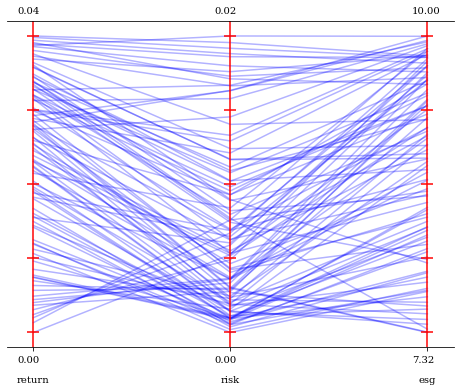
\includegraphics{pcpPlot}
\end{figure}

Figure 2 is the horizontal bar chart containing the mean weight given to each stock from the 200 solutions. From the plot it's clear that some stocks like ASML.AS were profitable choices and most stocks had either very small weights or they weren't included. 

\begin{figure}[H]
\caption{mean weight values}
\hspace*{-1.5cm}
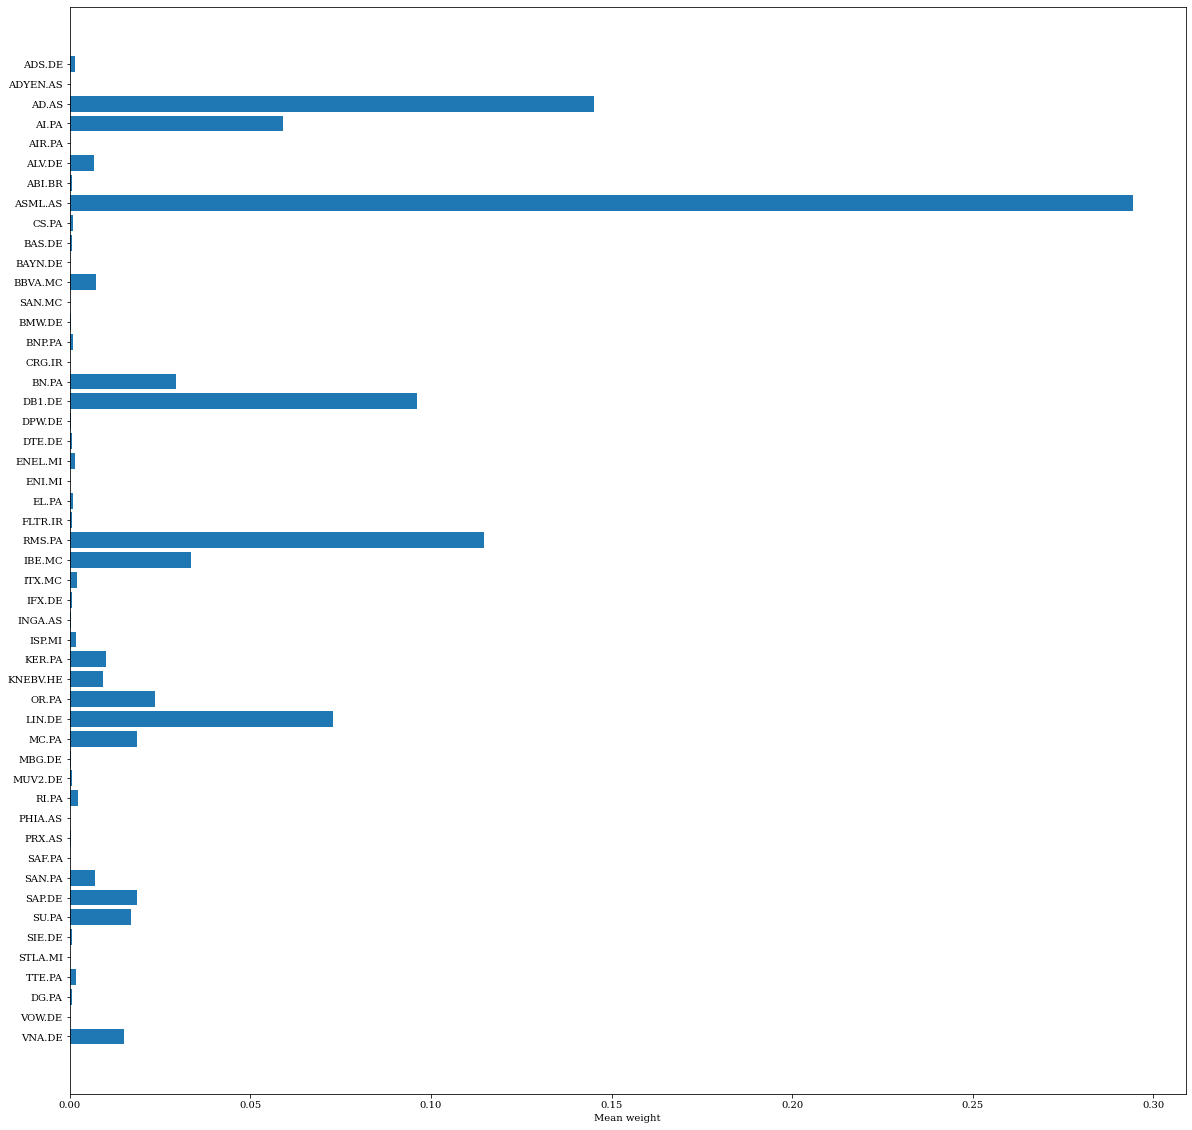
\includegraphics[scale=0.45]{meanW}
\end{figure}

The final solution was picked using Nautilus navigator. The table 2 contains the stocks included and their weights. The portfolio has expected increase in value of 3.2\% with 0.9\% risk and its ESG score is 8.7/10. The source code and the results are available at \url{https://github.com/juanrein/opt/tree/main/dataopt/final_project}.

\begin{table}[H]
\begin{tabular}{| c | c |}
\hline
stock & weight\\
\hline
AD.AS & 0.37\\
AI.PA & 0.05\\
ASML.AS & 0.38\\
RMS.PA & 0.07\\
LIN.DE & 0.03\\
MC.PA & 0.02\\
SU.PA & 0.04\\
TTE.PA & 0.02\\
VNA.DE & 0.02\\
\hline
\end{tabular}
\caption{Final solution stocks and weights}
\end{table}


\printbibliography %Prints bibliography

\end{document}
